\documentclass{article} % For LaTeX2e
\usepackage{nips14submit_e,times}
\usepackage{cite}
\usepackage{enumitem}
\usepackage{algorithm,algorithmicx}
\usepackage[noend]{algpseudocode}
\usepackage{url,graphicx,amsmath}
\usepackage{caption}
\usepackage[caption=false]{subfig}
%\documentstyle[nips14submit_09,times,art10]{article} % For LaTeX 2.09
\usepackage[pagebackref=true,breaklinks=true,letterpaper=true,colorlinks,bookmarks=false]{hyperref}

\title{Recruitment Analytics: Predict Applicant Behavior from Sparsely Labeled Application History}

\author{
%XIN LIN \\
%Department of Computer Science\\
%University of Texas at Austin \\
%Austin, TX 78705 \\
%\texttt{jimmylin@utexas.edu} \\
%\And
%Coauthor \\
%Affiliation \\
%Address \\
%\texttt{email} \\
%\AND
%Coauthor \\
%Affiliation \\
%Address \\
%\texttt{email} \\
%\And
%Coauthor \\
%Affiliation \\
%Address \\
%\texttt{email} \\
%\And
%Coauthor \\
%Affiliation \\
%Address \\
%\texttt{email} \\
%(if needed)\\
}

% The \author macro works with any number of authors. There are two commands
% used to separate the names and addresses of multiple authors: \And and \AND.
%
% Using \And between authors leaves it to \LaTeX{} to determine where to break
% the lines. Using \AND forces a linebreak at that point. So, if \LaTeX{}
% puts 3 of 4 authors names on the first line, and the last on the second
% line, try using \AND instead of \And before the third author name.

\newtheorem{remark}{Remark}
\newcommand{\fix}{\marginpar{FIX}}
\newcommand{\new}{\marginpar{NEW}}

\nipsfinalcopy % Uncomment for camera-ready version

\begin{document}


\maketitle

\section{Introduction}

\section{Formulation}
In this project, the task of predicting" apply" behaviors of given users can
be formulated as a recommendation problem. Such formulation naturally
gives rise to the matrix completion techniques. The optimization subsection
gives detailed illustration of the regular matrix completion problem and the
recently emerging inductive matrix completion problem. Besides, common
statistics for model evaluation in recommendation problem are given in the
assessment section. 

\subsection{Optimization}
% Intro to matrix completion
We will start from the classic (binary) matrix completion problem. What
follows is the one-class matrix completion problem, arised from practical
needs. Then we will transit to the fashioned inductive matrix completion,
which elegantly incorporate the features of users and jobs and address cold
startup problem in the meanwhile. 

\subsubsection{Classic Matrix Completion}
% 2.2 latent factor model 
The latent factor model has an underlying assumption: the real exact rating matrix are
low-rank matrix. That is, the derived low-rank matrix can exactly recover the
real rating matrix. By modelling target rating variable as 
\begin{align}
    R_{ij} = U_i^T V_j 
\end{align}
Then we are able to employ least square cost to approximate the presumed low-rank
matrix $R$ to the real rating matrix $A$: 
\begin{equation}
    \begin{aligned}
        &\min_{U,V} 
        && \sum_{(i,j)} (A_{ij} - U_i^T V_j)^2
        + \frac{\lambda}{2}(||U||_F^2 + ||V||_F^2)
    \end{aligned}
\end{equation}
where $|| \cdot ||_F$ denotes Frobenius norm, $A_{i,j}$ is the observed
ground-truth entry and $\Omega$ is the index set of entries that are observed
as positive $+1$ or negative $0$. 

\subsubsection{One-Class Matrix Completion}
\begin{equation}
    \begin{aligned}
        &\min_{U,V} 
        && \sum_{(i,j)\in \Omega} (1 - U_i^T V_j)^2
        + \frac{\lambda}{2}(||U||_F^2 + ||V||_F^2)
    \end{aligned}
\end{equation}
%\begin{remark}
%    Since some jobs have fairly limited number of previous history, then
%    One-Class Matrix Completion is expected to have bad performance.
%\end{remark}
\subsubsection{Inductive Matrix Completion}
% brief math introduction
Formulate the problem as that of recovering a low-rank matrix $W_*$ using
observed entries $R_{ij} = x_i^T W_{*} y_j$ and the user/job feature vectors $x_i$, $y_j$. By
factoring $W = U V^T$ , we see that this scheme constitutes a bi-linear
prediction $(x^T U_{*})(V_{*} y)$ for a new user/job pair $(x, y)$.
\begin{equation}
    \begin{aligned}
        &\min_{U,V} &&\sum_{(i,j)} (A_{ij} - x_i^TUV^Ty_j)^2 
        + \frac{\lambda}{2}(||U||_F^2 + ||V||_F^2)
    \end{aligned}
\end{equation}
% break through: dhillon's paper - inductive matrix completion
According to \cite{jain2013provable}, under standard set of assumptions,
the alternating minimization provably converges at a linear rate to the global
optimum of two low-rank estimation problems: a) RIP measurements based general
low-rank matrix sensing, and b) low-rank matrix completion. A more recent
paper \cite{natarajan2014inductive} in bioinformatics demonstrated successful
application of such inductive matrix completion
framework on gene-disease analytics.

\subsubsection{One-Class Inductive Matrix Completion}
\begin{equation}
    \begin{aligned}
        &\min_{U,V} &&\sum_{(i,j)\in\Omega} (1 - x_i^TUV^Ty_j)^2 
        + \frac{\lambda}{2}(||U||_F^2 + ||V||_F^2)
    \end{aligned}
\end{equation}

\subsubsection{One-Class Inductive Matrix Completion with Biases}
\begin{equation}
    \begin{aligned}
        &\min_{U,V} &&(1-\alpha) \sum_{A_{ij}=1} (1 - x_i^TUV^Ty_j)^2 +
        \alpha \sum_{A_{ij}=0} (0 - x_i^TUV^Ty_j)^2 + \frac{\lambda}{2}(||U||_F^2 + ||V||_F^2)
    \end{aligned}
\end{equation}

%\subsection{One-Class Inductive Matrix Completion with kernel method}
%% 3.2 propose kernel-based inductive matrix completion?
%One possible enhancement for above inductive matrix completion is to
%extend our consideration from the linear association between features and
%latent factors to an version that accepts non-linear association.
%By this intuition, we can name this approach as 
%    {\it Kernel-based Inductive Matrix Completion}.
%By taking into account non-linear relations between designed features and hidden
%topics (shared latent factors), the space of latent factors can be largely
%expanded and then it would be more likely to automatically detect latent
%factors with higher quality. 
% 
%\subsection{One-Class Inductive Matrix Completion with pre-clustering}
\subsection{Assessments}
In this research project, we employ Recall-Precision curve and MAP@N curve to 
asess and visually present the accurate performance of a particular model. 
\subsubsection{Recall-Precision Curve}
% precision and recall definition
In pattern recognition and information retrieval with binary classification,
precision, a.k.a. positive predictive value, is the fraction of retrieved
instances that are relevant, while recall, a.k.a. sensitivity, is the
fraction of relevant instances that are retrieved. According to the general
definition, the precision and recall for one query in this recommendation problem can be
formulated as 
\begin{align}
    \text{precision} &=  \frac{\text{number of jobs one user should appply and also
            recommended}}{\text{number of jobs recommended to the user}} \\
    \text{recall} &= \frac{\text{number of jobs one user should appply and
            also recommended}}{\text{number of jobs one user should apply}}
\end{align}
% TODO: advantage of rp curve

% weakness of rp curve
Nevertheless, precision and recall are single-value metrics that take no ordering information
into account. Thus, the recall-precision curve cannot assess performance of a
model from the "order-does-matter" perspective.
\subsubsection{MAP@N Curve}
For job recommendation system, it is supposed to return a ranked sequence of
suitable jobs for users to apply. Therefore, it is desirable to also consider the
order in which the returned jobs are presented. The mean average precision
(MAP) does vary in terms of the order of returned jobs and thus cumulative
MAP@N curve can serve as an effective tool to visualize the quality of queried
recommendations for both ordering and accuracy.

% AP
The prerequisite of computing mean average precision is to figure out average
precision (AP) for each queried user. The average precision at certain
position $N$ is defined as
\begin{align}
    \text{AP@N} &= \sum_{i=1}^N \text{precision}(i) \cdot \Delta \text{recall} (i)
\end{align}

% MAP
Taking the mean of average precision at the corresponding position for all
queried users derives the mean average precision .
\begin{align}
    \text{MAP@N} &= \frac{1}{| \Psi |} \sum_{u \in \Psi}
    \text{AP}_u\text{@N}
\end{align}
where $\Psi$ indicate the collection of queried users and $|\cdot|$ returns
the cardinality of a set.

% MAP@N remark

\section{Implementation}
\subsection{Algorithm}
% algorithm presentation
\newcommand{\xii}{\boldsymbol{x}_i}
\newcommand{\yj}{\boldsymbol{y}_j}
The algorithmic description for {\it One-class Inductive Matrix Completion
    with biased weight} are shown in Algorithm \ref{alg:AltMin}.  
\begin{algorithm}
    \caption{Alternating Minimization for One-Class Inductive Matrix Completion with Biases}
    \label{alg:AltMin}
    \begin{algorithmic}[1]

\State \textbf{INPUT}: \\ \ \ a) sparse matrices $X$ and $Y$ that denote features of users
and jobs respectively. \\ \ \ b) matrix $A$ that denotes partial observation
of "apply" association with observed index set $\Omega$ \State \

\State Initialize $U_{(0)}$ and $V_{0}$ by uniform randomization
\State \textbf{Do}  
\State \ \ \
$V_{(k+1)}$ = argmin $(1-\alpha) \sum_{(i,j) \in \Omega} 
    (1- \xii^T U_{(k)} V_{(k)}^T \yj)^2 
    + \alpha \sum_{(i,j) \not \in \Omega} (0 - \xii^T U_{(k)} V_{(k)}^T \yj)^2$

\State \  \
$U_{(k+1)}$ = argmin $(1-\alpha) \sum_{(i,j) \in \Omega}
    (1-\xii^T U_{(k)} V_{(k+1)}^T \yj)^2 +
    \alpha \sum_{(i,j) \not \in \Omega}
    (0-\xii^T U_{(k)} V_{(k+1)}^T \yj)^2$
\State \textbf{Until} Convergence. 
%\State Predict values for missing entries: for some $ (i,j) \not \in \Omega$,
%\State 
%\ \  \ $R_{ij} = 1,\ \text{for top } r $ items
%\State 
%\ \  \ $R_{ij} = 0,\ \text{otherwise}$

\State \

\State \textbf{OUTPUT: } \\ 
\ \ a) Model Parameter $ U_{*}$ and $V_{*}$ 
\end{algorithmic}
\end{algorithm}

%{{{ Newton Conjugate descent Method
\begin{algorithm}
    \caption{Newton Conjugate Descent Subroutine}
    \label{alg:newton}
    \begin{algorithmic}[1]

\State \textbf{INPUT}: \\ \ \ a) 
\\ \ \ b) 
\State \

\State Initialize $U_{(0)}$ and $V_{0}$ by uniform randomization
\State \

\State \textbf{OUTPUT: } \\ 
\ \ a) Model Parameter $ U_{*}$ and $V_{*}$ 
\end{algorithmic}
\end{algorithm}
%}}}

%{{{ Prediction Routine
\begin{algorithm}
    \caption{Prediction}
    \label{alg:prec}
    \begin{algorithmic}[1]

\State \textbf{INPUT}: \\ \ \ a) sparse matrices $X$ and $Y$ denote features of users
and jobs. \\ \ \ b) matrix $A$ denotes partial observation of application
association with observed index set $\Omega$
\State \

\State Initialize $U_{(0)}$ and $V_{0}$ by uniform randomization
\State \

\State \textbf{OUTPUT: } \\ 
\ \ a) Model Parameter $ U_{*}$ and $V_{*}$ 
\end{algorithmic}
\end{algorithm}
%}}}

%{{{ Preclustering
\begin{algorithm}
    \caption{Preclustering}
    \label{alg:preclustering}
    \begin{algorithmic}[1]

\State \textbf{INPUT}: \\ \ \ a) sparse matrices $X$ and $Y$ that denote features of users
and jobs respectively. \\ \ \ b) matrix $A$ that denotes partial observation
of "apply" association with observed index set $\Omega$ \State \

\State Initialize $U_{(0)}$ and $V_{0}$ by uniform randomization
\State \textbf{Do}  
\State \ \ \
$V_{(k+1)}$ = argmin $(1-\alpha) \sum_{(i,j) \in \Omega} 
    (1- \xii^T U_{(k)} V_{(k)}^T \yj)^2 
    + \alpha \sum_{(i,j) \not \in \Omega} (0 - \xii^T U_{(k)} V_{(k)}^T \yj)^2$

\State \  \
$U_{(k+1)}$ = argmin $(1-\alpha) \sum_{(i,j) \in \Omega}
    (1-\xii^T U_{(k)} V_{(k+1)}^T \yj)^2 +
    \alpha \sum_{(i,j) \not \in \Omega}
    (0-\xii^T U_{(k)} V_{(k+1)}^T \yj)^2$
\State \textbf{Until} Convergence. 
%\State Predict values for missing entries: for some $ (i,j) \not \in \Omega$,
%\State 
%\ \  \ $R_{ij} = 1,\ \text{for top } r $ items
%\State 
%\ \  \ $R_{ij} = 0,\ \text{otherwise}$

\State \

\State \textbf{OUTPUT: } \\ 
\ \ a) Model Parameter $ U_{*}$ and $V_{*}$ 
\end{algorithmic}
\end{algorithm}
%}}}


\subsection{Practical Issues}
\textbf{Bias}. Bias parameter $\alpha \in (0, 1)$ is the weight to balance
optimization objective between observed and missing labels. Note that we can
simply set $\alpha = 1$ to solve unbiased version of one-class inductive matrix completion.

\textbf{Initialization}. Randomizing all components of $U_{(0)}$ and
$V_{(0)}$ to uniform distribution over $(0, 1)$ works well in our
experimentation. 

\textbf{Optimization}.
During each stage of alternating minimization, standarded conjugate gradient method is
employed to solve least square problem. 

\section{Experiment I: Feature Extraction} % 3 pages
\subsection{Dataset}
% introduce experimented data set
The dataset utilized in this experimental project comes from a Job
Recommendation Challenge posted on
\href{http://www.kaggle.com/c/job-recommendation/data}{Kaggle.com}. The
provider of this dataset is
\href{http://www.careerbuilder.com/}{CareerBuilder.com}, one of the biggest
job recommendation service providers. This particular dataset, sized of several
Gigabytes, contains 389,708 featured users, 1,092,096
characterized jobs and 1,603,111 application records that are divided into
training and testing split.  In this section, we will at first provide the
fundamental introduction to these three basic elements: User, Job,
Application. And then explanation are illustrated about temporal separation (concept of
window) and designed distribution for user, job and application. 

% show details each record of user
As the most essential component of job recommendation system, users are
recorded by UserID, WindowID, Split, City, State, Country, ZipCode,
DegreeType, Major, GraduationDate, WorkHistoryCount,
TotalYearsExperience, CurrentlyEmployed, ManagedOthers, ManagedHowMany.
{\it UserID} refers to the nubmering index of that indicated user.  
{\it WindowsID} is about the timing period in which this particular
applicaiton about user happened. 
{\it City, State, Country, and ZipCode} are related to the living place of
that user. 
What follows are the achievements in school. 
{\it DegreeType} shows the highest degree that user has gained from school,
{\it Major} presents the field of his/her speciality and 
{\it GraduationDate} reveals when he/she gained the highest degree.
Working and management experience comes next.
{\it WorkHistoryCount} represents how many previous jobs one has had and
{\it TotalYearsExperience} represents how many years one has been involved in
occupation. 
{\it CurrentlyEmployed} and {\it ManagedOthers} are both binary values,
indicating whether one was currently on his/her job and whether he has been in
certain management position. 
{\it ManagedHowMany} implies his management power and capability, that is, the maximum number
of people he/she has managed before.

% show details each record of job
When it comes to information of every individual job, fields like JobID,
WindowID, Title, Description, Requirements, City, State, Country, Zip5,
StartDate, EndDate are provided.
{\it JobID} is the identifying number for each particular job. 
{\it WindowID} captures the same semantics as it is in a user record --
involved timing period of one job.
{\it Title} is the name of position sepcified by corresponding corporation, which
can be significantly important since it reflects relative position and power
in one company's hierarchy. 
Description and Requirements are both textual characterization
over each particular job. 
{\it Description} provides a
characteristic overview of one particular job. 
{\it Requirements} can be
viewed the basic expectation of hiring company towards the job applicants.
Similarly to the record of each individual user, every job also has location
information, such as {\it City, State, Country, ZipCode}. 
Besides, {\it StartDate} and {\it EndDate} shows the timing information of one job,
i.e. on which day it starts and ends. 

% show details each record of application
As to each instanced record of application, the dataset contains information
about the UserID, WindowID, Split, ApplicationDate, and JobID. 
{\it UserID} is indexing number of the user who applied for particular job,
indexed by {\it JobID}. 
{\it WindowID} implies the timing period of that application event, while
{\it ApplicationDate} presents the specific date of application event. 
And {\it Split} labelled in which division (training or testing set) that
piece of application was placed.

% explain the window ID
Next presented was the overall explanation about timing design of dataset. In
outline, all application instances span 13 weeks. All the job applications are
split into 7 groups, with each group representing a 13-day window. Each 13-day
window is split into two parts: The first 9 days are the training period, and
the last 4 days are the test period. The graphical representation
demonstrating such splits is illustrated below.
\begin{figure}[h]
    \begin{center}
        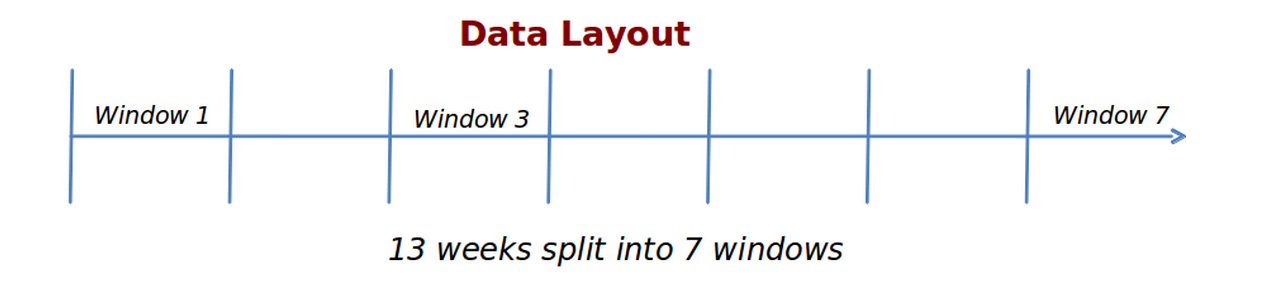
\includegraphics[width=4.3in,height=1.4in]{./fig/datalayout.png}
        \caption{Illustrating Diagram for Temporal Separation of the Dataset}
    \end{center}
\end{figure}

Note that each user and each job posting is randomly assigned to exactly one window.
Each job is assigned to a window with probability proportional to the time it
was live on the site in that window. Each user is assigned to a window with
probabilty proportional to the number of applications they made to jobs in
that window. As shown in the figure below, User1 only made submissions to jobs in
Window 1, and so was assigned to Window 1 with probability 100\%. User2,
however, made submissions to jobs in both Window 1 and Window 2, and so may
have been assigned to either Window1 or Window2.

\begin{figure}[h]
    \begin{center}
        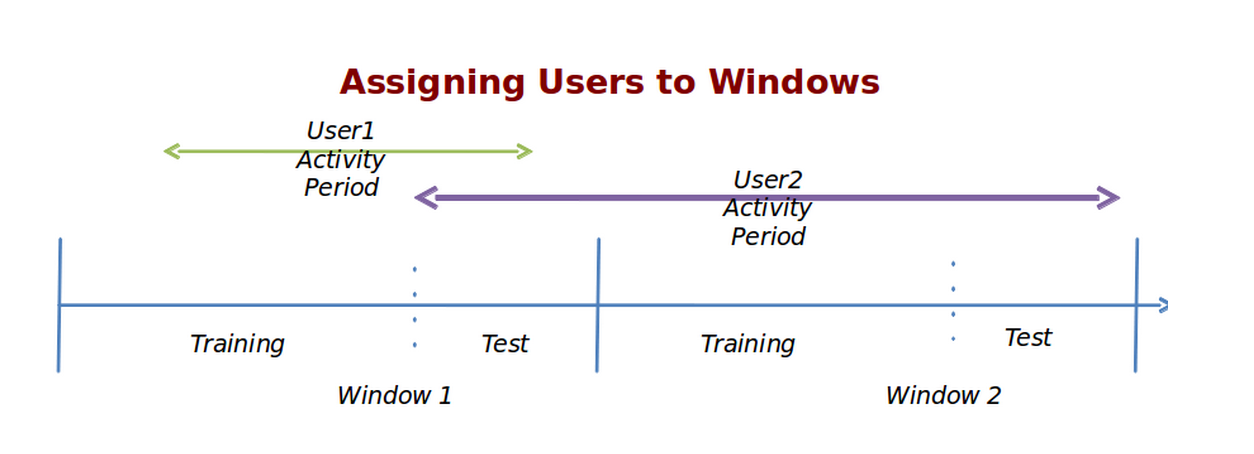
\includegraphics[width=4.3in,height=1.8in]{./fig/assignusertowindows.png}
        \caption{Explanation for user distribution}
    \end{center}
\end{figure}

In each window, all the job applications that users in that window made to
jobs in that window during the 9-day training period. 
And with each window, users have been split into two groups, {\it Test group}
and {\it Train group}. The Test users are those who made 5 or more
applications in the 4-day test period, and the Train users are those who did
not.

For each window, the task of prediction is which jobs in that window the Test
users applied for during the window's test period. Note that users may have
applied to jobs from other windows as well, but the only thing needed to be
predicted is which jobs they applied to in their own windows.

% TODO:some key observation from dataset

\subsection{Preprocessing} % ways to preprocessing
Preprocessing, as the earliest step for any machine learning
experimentation, is extremely important in that it, as a role of filter, 
process the raw data and then generates what is later employed by human-design
AI system. From this perspective, any inconsistent or invalid processing would
cause devastating effects for the entire system.

% 0. instance subsetting
{\bf Instance Subsetting}.
Since there are huge quantities of users and jobs, our experiment only
exploits the first part of dataset (WindowsID = 1) for computational
convenience. Another benefit for such instance subsetting is to temporarily
put aside the temporal dynamics, that is, disregard the impact of timing
variable for now. And the investigation over how to accommodate the designed system
to the entire dataset can be deferred to later study.

% 1. binary encoding of discrete value
{\bf Binary Encoding Scheme}.
For all nominal attributes, we represent every of them as a collection of binary
variables. For example, DegreeType, indicating the highest
degree obtained by one user, has five possible values: None, High
School, Bachelor, Master, PhD. We have five binary variables indicating if one
user has highest degree on None, High School, Bachelor, Master, PhD
respectively. Other examples of such nominal attributes in this application
prediction problem are Zip5, City, State and Country. 
One advantage of such processing lies in multi-valued features, like Major.
Some people may be double-major or even three-major. 
In these cases, no conflict would occur if we apply take binary encoding
scheme. However, the binary encoding scheme will significantly augment the scale of
learning task since some nominal attributes have huge domain dimensionality.
Hence, it is unavoidable to leave out redundant attributes. 

% 2. feature subsetting (user, job, application)
{\bf Attributes Subsetting}.
To simplify initial setup of this machine learning experimentation, we
manually left out some three categories of attributes. First category is
semantically meaningless information. On top of that, those attributes that may contribute to
application prediction (slightly higher accuracy) but overwhelmingly enlarge
the scale of learning (significantly lower speed) are also eliminated for now.
Zip5 is the most illustrative example for this type of attribute.
Another set of attributes are disregarded because we are incapable of
modelling these relevant factors. For example, temporal dynamics (i.e. {\it
    StartDate and EndDate} of job) are not planned to be captured in our
current design. 

% 3. processing textual data (description, requirements)
%% (present procedure)
{\bf Efficient Representation of Textual Data}.
The ways to process textual data are important because we hope to narrow the
scale of numerical representation for these texts.  The sequential procedures
of processing raw text data are specified as follows:
\begin{enumerate}[label=(\roman*)]
  \item{Convert all terms into lowercase.}
  \item{Eliminate stop words.}
  \item{Annihilate all meaningless terms with particular forms, i.e.
          timestamps, datestamps, IP addresses, phone numbers and webpage link}
  \item{Remove all punctuations.}
  \item{Check validity of words.}
  \item{Acquires linguistic stemmes for each tokens. This step also removes
          plurals and tenses.}
\end{enumerate}
%% (present statistics of product)
As a consequence of applying above transformations, {\bf 12841}
keywords (distinct vocabularies) are obtained. 

% 4. data format of preprocessing product 
{\bf Preprocessing Products}.
Through preprocessing, we generate three data files for later machine learning
algorithm: {\it win1\_Users.sparse, win1\_Jobs.sparse and win1\_Apps.sparse}.
Within {\it win1\_Users.sparse}, there are $77060$ users with $1416$ features per
user. {\it win1\_Jobs.sparse} maintained records of $285515$ jobs, each of
which has $12841$ features for now. {\it win1\_Apps.sparse} contains a sparse
matrix with dimensionality $77060\times285515$.

{\bf Storage Format} Note that all numerics generated by preprocessing procedure are restored as libSVM
format in that the generated features for user and job have huge extent of sparsity. 
Specifically, for every job or user contained in win1\_Users.sparse,
win1\_Jobs.sparse, the representation of each object is as follows:
\begin{center}
    feature\_index:feature\_value \ feature\_index:feature\_value .... 
\end{center}
On the other hand, the representation for each application instance is slightly different,
but still in standarded LibSVM format. 
\begin{center}
    apply\_or\_not 0:user\_index 1:job\_index
\end{center}

\section{Experiment II: Basic Parameters} % 4 pages

\subsection{Effects of Rank $K$}
We trace the main term in training stage.
\begin{figure}[hp]
    \centering
    \captionsetup{justification=centering}
    \subfloat{ 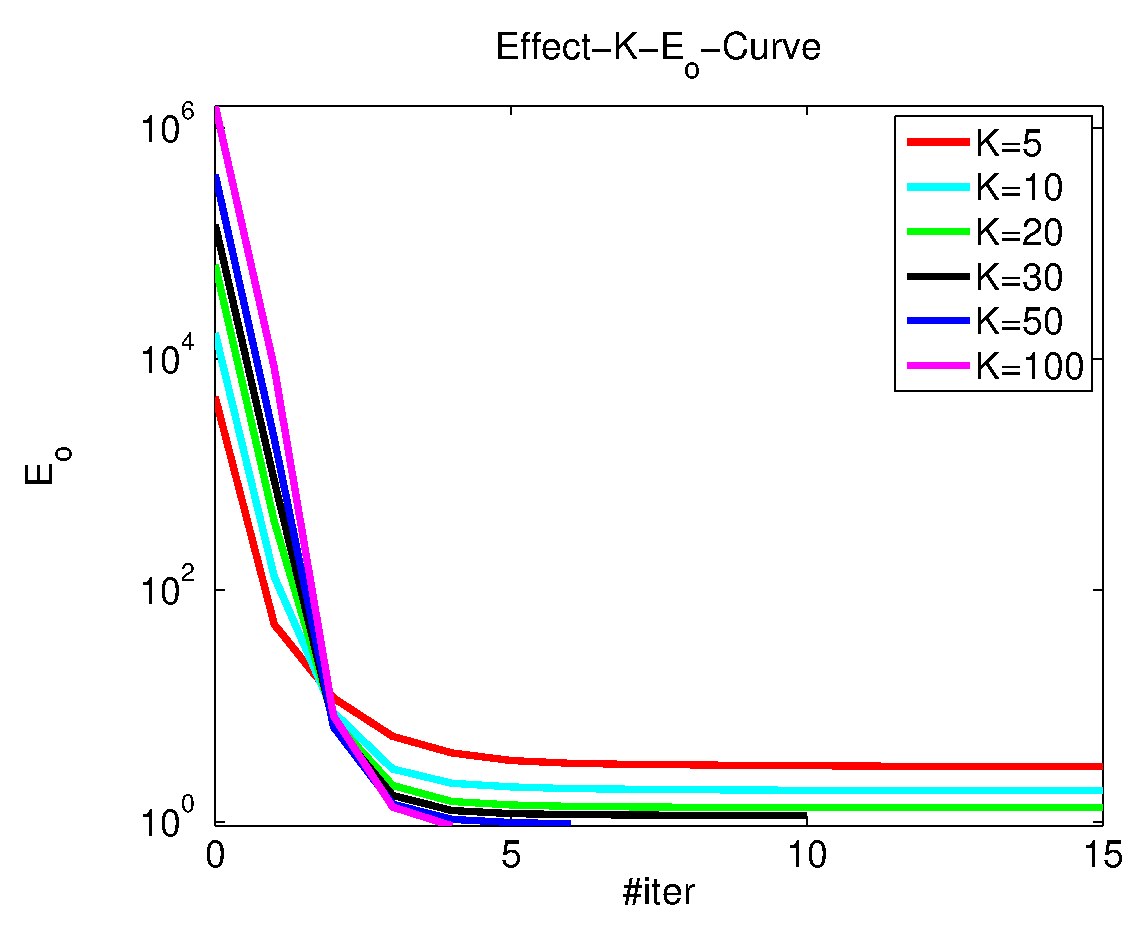
\includegraphics[width=65mm]{Effect_K/E_o_Curve.eps} }
    \subfloat{ 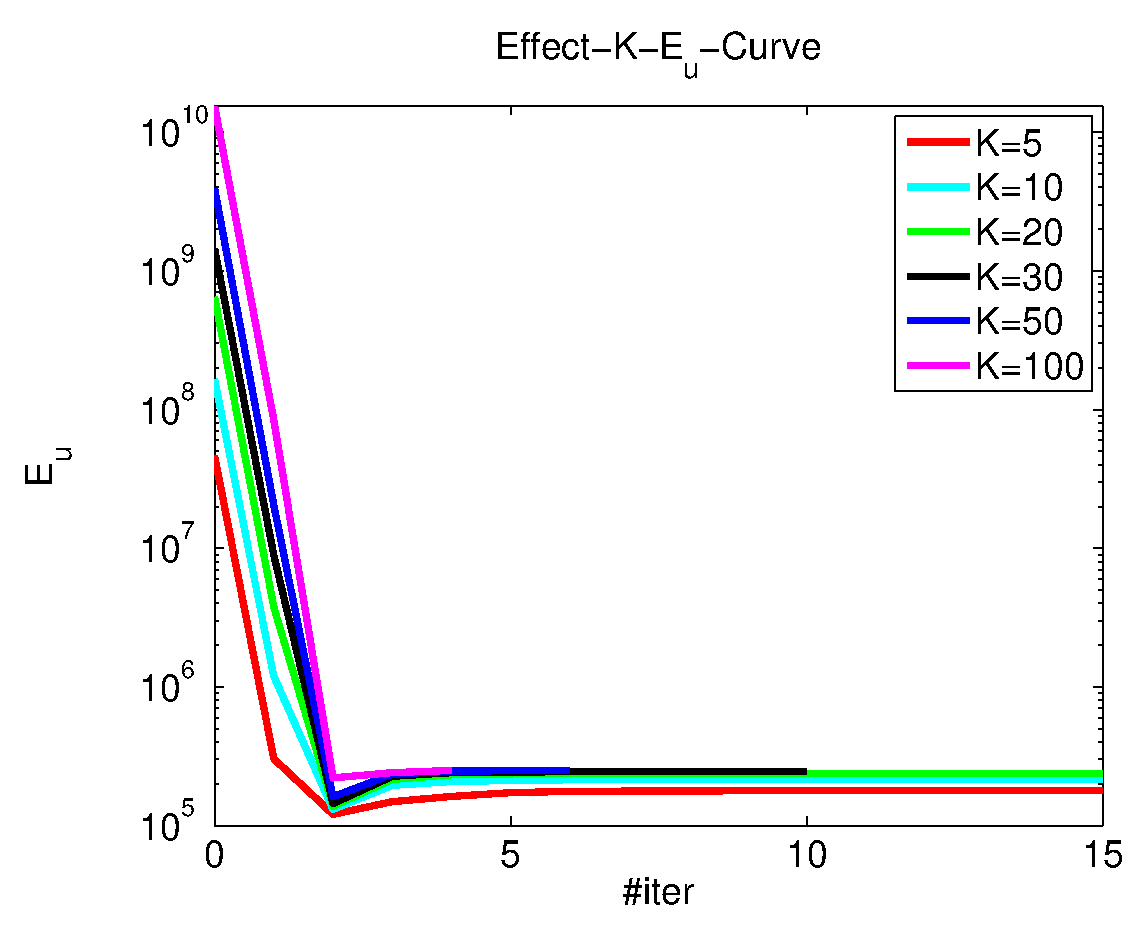
\includegraphics[width=65mm]{Effect_K/E_u_Curve.eps} }
    \caption{Trace $E_o$ and $E_u$ between the trained models with various
        $K=5,10,20,30,50$. \newline
        Left: $E_o$ Curve. Right: $E_u$ Curve. } 
    \label{EffectK:Eo_Eu}
\end{figure}

The performance evaluation is as follows.
\begin{figure}[hp]
    \centering
    \captionsetup{justification=centering}
    \subfloat{
        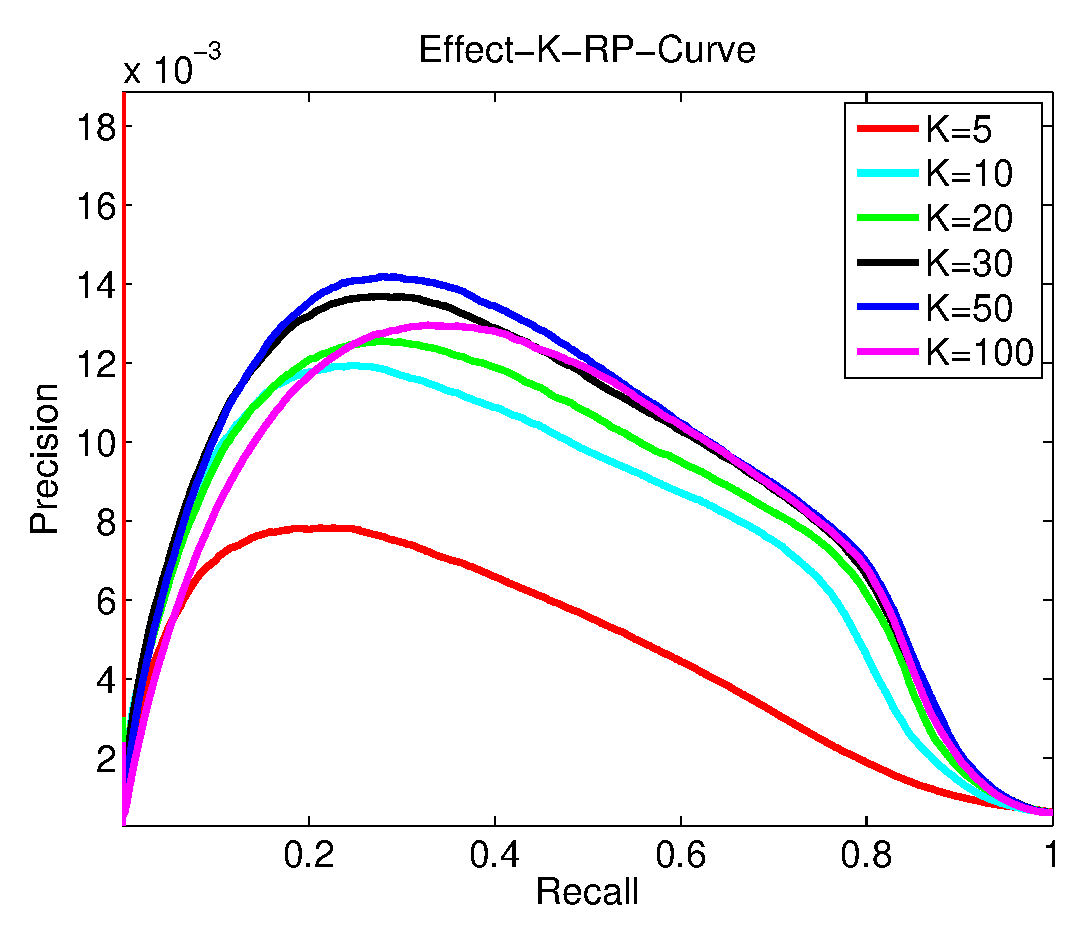
\includegraphics[width=65mm]{Effect_K/RP_Curve.eps}
    }
    \subfloat{
        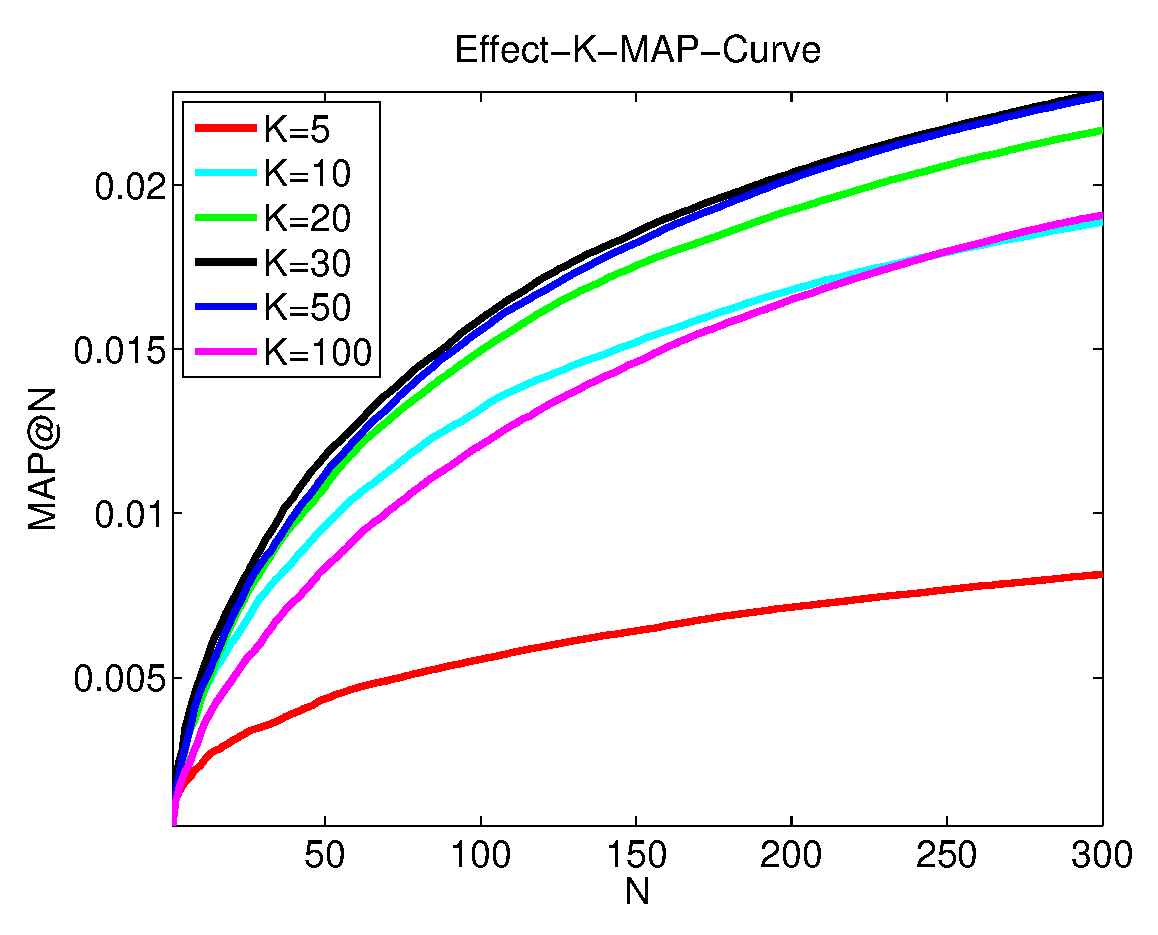
\includegraphics[width=70mm]{Effect_K/MAP_Curve.eps}
    }
    \caption{Performance Comparison between the trained models with various
        $K=5,10,20,30,50$.  Left: Precision-Recall Curve. Right: MAP@N Curve. }
    \label{EffectK:RP_MAP}
\end{figure}

\subsection{Effects of Bias Weight $\alpha$}

\subsection{Effects of Regularization Parameter $\lambda$}

\subsection{Effects of Early Stopping}


\section{Experiment III: Revisits Feature Engineering}
\subsection{Best-Tuned Setting}

\subsection{Principal Component analysis}


\section{Experiment IV: Pre-clustered Matrix Completion}

\subsection{Results}



\begin{figure}[h]

    \caption{Precision v.s. Recall Comparison between models with
        $\lambda=\lambda_0, \lambda_1,\lambda_2, \lambda_3$ }
\end{figure}

\begin{figure}[h]

    \caption{Precision v.s. Recall Comparison between various models with
        different preprocessed data}
\end{figure}

\section{Conclusions}
% one concluding paragraph
Features do provide supervision for recognizing the pattern of new users. 

% in the future
Future work can be extended to modeling time-series recommendation problem by
means of one-class inductive matrix completion. 

%\subsubsection*{References}
\bibliography{main}{}
\bibliographystyle{plain}


\end{document}
